%!TEX root = ../../main.tex

\chapter{Realisierung}

Nachdem im theoretischen Teil die Grundlagen, Herausforderungen und geeigneten Visualisierungstechniken für Knowledge Graphen erarbeitet wurden, widmet sich dieses Kapitel der praktischen Umsetzung der gewonnenen Erkenntnisse. Ziel ist es, ein System zu entwickeln, welches dazu in der Lage ist einen Knowledge Graphen zu visualisieren und den Anforderungen, die sich aus dem Theorieteil ableiten lassen, gerecht zu werden. Das System wird im Folgenden Kapitel als Graph Visualizer bezeichnet.

\section{Konzept}

In diesem Abschnitt wird das Konzept für die Umsetzung des Graph Visualizers entwickelt. Auf Basis des theoretischen Teils, werden zunächst die funktionalen und nicht-funktionalen Anforderungen an den Graph Visualizer analysiert. Anschließend werden die geeigneten Diagrammarten ausgewählt und die notwendigen Technologien festgelegt. Das erarbeitete Konzept bildet die Grundlage für die nachfolgende Implementierung und gewährleistet, dass der Graph Visualizer sowohl den technischen als auch den benutzerseitigen Anforderungen entspricht. Dabei wird besonders darauf geachtet, dass die Architektur des Systems flexibel und erweiterbar gestaltet ist, um zukünftige Anpassungen und Erweiterungen zu ermöglichen.

\subsection{Anforderungsanalyse}
\label{realization:requirements}

In diesem Abschnitt werden die spezifischen Anforderungen an den Graph Visualizer untersucht und definiert. Dabei wird zwischen funktionalen und nicht-funktionalen Anforderungen unterschieden. Die funktionalen Anforderungen beschreiben die konkreten Funktionen, die der Graph Visualizer erfüllen muss, wie etwa die Visualisierung von Knowledge Graphen, die Interaktivität und die Anpassungsfähigkeit der Darstellung. Die nicht-funktionalen Anforderungen hingegen befassen sich mit Aspekten wie Performance, Skalierbarkeit, Benutzerfreundlichkeit und Sicherheit. Die Anforderungen werden aus den Erkenntnissen aus Kapitel \ref{theory} abgeleitet. Diese Analyse bildet die Grundlage für die Auswahl der geeigneten Technologien und die Entwicklung eines Systems, das den Erwartungen der Benutzer entspricht und gleichzeitig den technischen Herausforderungen gerecht wird.

\subsubsection{Funktionale Anforderungen}

Für dieses Projekt wurde festgelegt, dass der Graph Visualizer die Daten des DBpedia Graphen visualisieren soll. DBpedia ist eine umfassende Wissensdatenbank, die auf strukturierten Informationen aus Wikipedia basiert. Diese Datenquelle wurde ausgewählt, da sie einen großen, frei zugänglichen Knowledge Graphen zur Verfügung stellt. Die genauen Daten sind in diesem Projekt zweitrangig. Es geht darum mit welchen Techniken ein Knowledge Graph dargestellt werden kann und nicht darum welche Daten dargestellt werden.

Der Graph Visualizer muss in der Lage sein, Knowledge Graphen effektiv darzustellen. Dies umfasst die Fähigkeit, Knoten und Kanten zu rendern und unterschiedliche Visualisierungstechniken anzuwenden, um die Daten strukturiert und verständlich zu präsentieren. Die Visualisierung muss es ermöglichen, komplexe Netzwerke übersichtlich darzustellen und verschiedene Perspektiven auf die Daten anzubieten.

Ein wesentliches Merkmal des Graph Visualizer ist die Interaktivität. Benutzer müssen die Möglichkeit haben, mit dem Graphen zu interagieren, indem sie Knoten und Kanten auswählen, verschieben, vergrößern oder verkleinern. Darüber hinaus soll der Benutzer durch einfache Aktionen, wie Klicks oder Drag-and-Drop, den Graphen dynamisch erkunden und manipulieren können, um tiefere Einblicke in die Daten zu gewinnen.

Der Graph Visualizer soll es ermöglichen, die Darstellung der Graphen anzupassen. Dazu gehört die Fähigkeit, verschiedene Layouts auszuwählen, sowie die Darstellung des Graphen anzupassen. Diese Anpassungen sollen helfen, die Visualisierung an den spezifischen Kontext der Analyse anzupassen und die relevanten Informationen hervorzuheben.

Die eben definierten funktionalen Anforderungen sind in der Tabelle \ref{tab:realization:concept:funcreq} zusammengefasst.

\begin{center}
    \begin{longtable}{|l|p{4.5cm}|p{8cm}|}
        \caption{Funktionale Anforderungen an den Graph Visualizer}
        \label{tab:realization:concept:funcreq}  \\

        \hline
        \multicolumn{1}{|c|}{}            &
        \multicolumn{1}{ c|}{\textbf{FR}} &
        \multicolumn{1}{ c|}{\textbf{Bedeutung}} \\
        \hline
        \endhead

        \hline
        \endlastfoot

        FR01
        \label{FR01}
                                          &
        Darstellung von Daten aus DBpedia
                                          &
        Das System soll DBpedia als Datenquelle verwenden.
        \\
        \hline
        FR02
        \label{FR02}
                                          &
        Visualisierung von Knowledge Graphen
                                          &
        Das System soll dazu in der Lage sein einen Knowledge Graphen zu visualisieren.
        \\
        \hline
        FR03
        \label{FR03}
                                          &
        Interaktivität
                                          &
        Das System muss dem Nutzer verschiedene Möglichkeiten zu Interaktion bieten.
        \\
        \hline
        FR04
        \label{FR04}
                                          &
        Anpassbarkeit der Darstellung
                                          &
        Der Nutzer muss die Darstellung anpassen können.
        \\
    \end{longtable}
\end{center}

\subsubsection{Nicht-Funktionale Anforderungen}

Der Graph Visualizer muss eine hohe Reaktionsgeschwindigkeit aufweisen, insbesondere bei der Verarbeitung großer Datenmengen. Ladezeiten sollten minimiert und Interaktionen wie das Verschieben, Zoomen oder Auswählen von Knoten sollten ohne Verzögerungen durchgeführt werden können. Das System sollte in der Lage sein, selbst bei Netzwerken mit tausenden von Knoten und Kanten flüssig zu arbeiten.

Das System muss stabil und zuverlässig funktionieren. Es darf nicht zu Abstürzen kommen, selbst wenn es mit unerwarteten Eingaben oder sehr großen Datenmengen konfrontiert wird.

Der Graph Visualizer sollte auf verschiedenen Plattformen und Betriebssystemen lauffähig sein. Der Nutzer soll den Graph Visualizer von jedem gängigen System aus verwenden können.

Das System sollte leicht wartbar sein. Der Quellcode muss gut strukturiert sein, um zukünftige Anpassungen und Erweiterungen zu erleichtern. Ein modularer Aufbau des Systems ist wünschenswert, um einzelne Komponenten einfach austauschen oder aktualisieren zu können.

Die Benutzeroberfläche sollte intuitiv und leicht verständlich sein. Es sollten umfassende Hilfsmittel wie Tooltips zur Verfügung stehen.

Die eben definierten nicht-funktionalen Anforderungen sind in der Tabelle \ref{tab:realization:concept:nonfuncreq} zusammengefasst.

\begin{center}
    \begin{longtable}{|l|p{4.5cm}|p{8cm}|}
        \caption{Nicht-funktionale Anforderungen an den Graph Visualizer}
        \label{tab:realization:concept:nonfuncreq} \\

        \hline
        \multicolumn{1}{|c|}{}             &
        \multicolumn{1}{ c|}{\textbf{NFR}} &
        \multicolumn{1}{ c|}{\textbf{Bedeutung}}   \\
        \hline
        \endhead

        \hline
        \endlastfoot

        NFR01
        \label{NFR01}
                                           &
        Performance
                                           &
        Die Anwendung muss eine hohe Reaktionsgeschwindigkeit aufweisen und selbst bei Graphen mit tausenden Knoten flüssig arbeiten.
        \\
        \hline
        NFR02
        \label{NFR02}
                                           &
        Zuverlässigkeit
                                           &
        Das System muss stabil und zuverlässig funktionieren.
        \\
        \hline
        NFR03
        \label{NFR03}
                                           &
        Kompatibilität
                                           &
        Der Graph Visualizer sollte auf verschiedenen Plattformen und Betriebssystemen lauffähig
        sein.
        \\
        \hline
        NFR04
        \label{NFR04}
                                           &
        Wartbarkeit
                                           &
        Das System sollte leicht zu warten und erweitern sein.
        \\
        \hline
        NFR05
        \label{NFR05}
                                           &
        Benutzerfreundlichkeit
                                           &
        Die Benutzeroberfläche sollte intuitiv und leicht verständlich sein.
        \\
    \end{longtable}
\end{center}

\subsection{Vergleiche und Auswahl der Visualisierungstechniken}

In diesem Kapitel werden die verschiedenen Visualisierungstechniken, die im theoretischen Teil der Arbeit vorgestellt wurden, analysiert und verglichen. Ziel ist es, die am besten geeigneten Techniken für die Implementierung im Graph Visualizer auszuwählen. Die Auswahl der Techniken erfolgt mit Blick auf die in Kapitel \ref{realization:requirements} definierten Anforderungen. Dieses Kapitel ist in zwei Unterkapitel unterteilt. Das erste beschäftigt sich mit der Auswahl geeigneter Diagrammarten, während das zweite die spezifischen Visualisierungstechniken betrachtet, die für die Darstellung der Knowledge Graphen eingesetzt werden sollen.

\subsubsection{Diagrammarten}

Für die Implementierung des Graph Visualizer werden sowohl Node-Link-Diagramme als auch Adjazenzmatrizen ausgewählt, da beide Diagrammarten unterschiedliche Stärken aufweisen, die den spezifischen Anforderungen des Projekts gerecht werden. Node-Link-Diagramme werden aufgrund ihrer intuitiven Darstellung und Benutzerfreundlichkeit gewählt, da sie es ermöglichen, die Beziehungen zwischen Knoten direkt und visuell ansprechend zu repräsentieren. Diese Diagrammart unterstützt die Anforderung, ein System zu entwickeln, das auch für Nutzer ohne tiefgehende technische Kenntnisse leicht verständlich und bedienbar ist. Auf der anderen Seite bieten Adjazenzmatrizen eine effiziente Möglichkeit, dichte Netzwerke kompakt und übersichtlich darzustellen, was insbesondere für die Anforderung der Skalierbarkeit entscheidend ist. Adjazenzmatrizen eignen sich hervorragend zur Analyse komplexer und stark verbundener Netzwerke, indem sie Verbindungen in einer klar strukturierten Form präsentieren. Obwohl beide Diagrammarten für die Implementierung ausgewählt wurden, spielen sie nicht zusammen, sondern werden getrennt verwendet, um ihre jeweiligen Vorteile auszunutzen. In einem späteren Kapitel werden sie miteinander verglichen, um zu evaluieren, welche der beiden Methoden für bestimmte Anwendungsfälle besser geeignet ist und wie sie sich in der praktischen Anwendung bewähren. Hierarchische Layouts hingegen werden nicht berücksichtigt, da ein Knowledge Graph typischerweise nicht hierarchisch ist und solche Layouts daher die komplexen, nicht-linearen Strukturen eines Knowledge Graphen nicht adäquat abbilden könnten.

\subsubsection{Visualisierungstechniken}

Für die Implementierung des Graph Visualizer wurden sorgfältig verschiedene Visualisierungstechniken ausgewählt, die den Anforderungen des Projekts am besten entsprechen und gleichzeitig die Grundlage für eine spätere Erweiterung des Systems bieten. Eine der zentralen Techniken ist die Graph Filterung, die sowohl in der Vorverarbeitung als auch während des Betriebs des Systems zum Einsatz kommt. Diese Technik ermöglicht es, irrelevante oder weniger wichtige Knoten und Kanten aus dem Graphen zu entfernen oder auszublenden, wodurch die Komplexität der Darstellung reduziert und der Fokus auf relevante Daten gelenkt wird. Dies ist besonders wichtig bei großen Netzwerken, da die Analyse solcher Netzwerke oft durch die schiere Menge an Informationen erschwert wird. Die interaktive Filterung, die es den Nutzern ermöglicht, den Graphen dynamisch an ihre Bedürfnisse anzupassen, trägt entscheidend zur Benutzerfreundlichkeit und Flexibilität des Systems bei. Zudem wird ein Force-Directed Layout implementiert, das sich durch seine intuitive Darstellung und die Möglichkeit der Anpassung aller Parameter durch den Nutzer auszeichnet. Diese Technik basiert auf physikalischen Modellen, die dafür sorgen, dass verwandte Knoten näher beieinanderliegen, was es dem Nutzer erleichtert, Cluster und Beziehungen im Netzwerk zu erkennen. Das Force-Directed Layout unterstützt die Anforderung, ein hochgradig interaktives und anpassbares System zu entwickeln, das auch komplexe Netzwerke verständlich darstellt. Ein weiterer wesentlicher Bestandteil des Graph Visualizer ist die Integration des Louvain-Algorithmus zur Clustererkennung. Dieser Algorithmus ist besonders für große Netzwerke geeignet und ermöglicht es, Cluster ohne vorherige Festlegung ihrer Anzahl zu identifizieren. Dies ist von besonderer Bedeutung für die Visualisierung von Knowledge Graphen, die in der Regel keine vorab bekannte Struktur aufweisen. Durch die Clustererkennung wird das Netzwerk in überschaubare Segmente unterteilt, was die Analyse erleichtert und die Skalierbarkeit des Systems verbessert. Andere im theoretischen Teil vorgestellte Techniken, wie das Edge Bundling oder die Fischaugen-Ansicht, werden aufgrund zeitlicher Einschränkungen nicht implementiert, obwohl sie ebenfalls nützlich sind. Der Fokus liegt auf den Methoden, die die Anforderungen am besten erfüllen und gleichzeitig die Grundlage für eine spätere Erweiterung des Systems bilden. Diese ausgewählten Techniken werden in späteren Kapiteln evaluiert, um ihre Effektivität und Eignung für die spezifischen Anforderungen des Graph Visualizer zu überprüfen und zu validieren.

\subsection{Technologieauswahl}

In diesem Abschnitt werden die Technologien beschrieben, die für die Implementierung des Graph Visualizer ausgewählt wurden. Die Wahl der Technologien basiert auf den Anforderungen, die in den vorherigen Kapiteln definiert wurden, und zielt darauf ab, ein robustes, flexibles und leistungsfähiges System zu schaffen, das die Visualisierung von Knowledge Graphen effektiv unterstützt.

\subsubsection{Frontend-Technologien}

Das Frontend des Graph Visualizer wird als \ac{SPA} realisiert. Dafür wurde Svelte als Framework gewählt, da es eine hohe Performance bietet und einfach von Einsteigern erlernt werden kann. Svelte ermöglicht es, reaktive Webanwendungen zu erstellen, bei denen die Benutzeroberfläche auf Benutzerinteraktionen reagiert. Um das Styling der Anwendung zu unterstützen, wird TailwindCSS eingesetzt. Ergänzend dazu wird DaisyUI verwendet, um die Entwicklung zu beschleunigen. DaisyUI ist eine auf TailwindCSS basierende UI-Komponentenbibliothek, die vorgefertigte Komponenten bereitstellt.

Für die Visualisierung der Graphen kommt D3.js zum Einsatz. D3.js ist eine JavaScript-Bibliothek, die für die Erstellung dynamischer und interaktiver Datenvisualisierungen entwickelt wurde. D3.js ermöglicht es, Daten in verschiedensten Formaten zu binden und diese durch Transformation des \ac{DOM} in komplexe Visualisierungen umzusetzen. Diese Flexibilität und dessen Verbreitung machen D3.js besonders geeignet für die Darstellung von Knowledge Graphen (vgl. \cite{d3js:Bostock}). Es gibt auch Alternativen zu D3.js, wie zum Beispiel Sigma.js, eine Bibliothek, die sich ebenfalls für die Darstellung von Netzwerken eignet und sich durch eine optimierte Performance für große Netzwerke auszeichnet. Sigma.js ist besonders dann nützlich, wenn der Fokus auf der schnellen und einfachen Darstellung von Netzwerken liegt, ohne die umfassende Anpassungsfähigkeit, die D3.js bietet (vgl. \cite{sigmajs:Jacomy}). Trotz der Vorteile von Sigma.js wurde sich für D3.js entschieden, da es weiter verbreitet ist und mehr online Ressourcen zur Verfügung stehen.

\subsubsection{Backend-Technologien}

Das Backend des Graph Visualizer wird mit ASP.NET Core entwickelt. Diese Wahl bietet mehrere Vorteile, darunter eine hohe Performance, Plattformunabhängigkeit und eine gut Unterstützung für moderne Webtechnologien. Darüber hinaus wurde ASP.NET Core aufgrund der bereits vorhandenen Kenntnisse und Erfahrungen mit diesem Framework ausgewählt. ASP.NET Core wird verwendet, um die Webseite auszuliefern. Gleichzeitig dient die Anwendung als Schnittstelle zur Verarbeitung und Bereitstellung der Knowledge Graphen-Daten. Das Backend ist dafür verantwortlich, die Daten aus der zugrunde liegenden Knowledge Graph-Datenquelle zu laden und diese über einen \ac{API} Endpunkt zur Verfügung zu stellen, der von der Svelte-Anwendung im Frontend abgerufen wird.

\subsubsection{Schnittstellen und Datenformate}

Die Kommunikation zwischen dem Frontend und dem Backend des Graph Visualizer erfolgt über eine RESTful \acs{API}, die vom Backend bereitgestellt wird. Das Backend, entwickelt mit ASP.NET Core, übernimmt die Aufgabe, die Daten aus einer externen Knowledge Graph-Datenquelle abzurufen. Diese Daten werden über einen \ac{SPARQL} Endpunkt im \ac{RDF} Format bezogen, einem Standardformat für die Darstellung von Metadaten in semantischen Netzwerken. Die ASP.NET Core Anwendung verarbeitet diese RDF-Daten und bringt sie in eine für das Frontend verständliche Form.

Die Svelte-Anwendung im Frontend erhält die aufbereiteten Daten dann im \ac{JSON} Format. \ac{JSON} bietet die nötige Flexibilität und Einfachheit, um komplexe Datenstrukturen, effizient darzustellen. Diese Struktur ermöglicht eine reibungslose Integration der Daten in die interaktiven Visualisierungen des Graph Visualizer. Durch diese Architektur wird eine klare Trennung zwischen den Datenformaten im Backend und der Datenpräsentation im Frontend gewährleistet, was die Wartbarkeit und Erweiterbarkeit des Systems verbessert.

\subsection{Zusammenfassung der Systemarchitektur}

Die Systemarchitektur des Graph Visualizer ist in die Client-Seite und die Server-Seite unterteilt. Auf der Client-Seite läuft das Frontend als Single Page Application im Browser des Users. Als JavaScript-Framework wird Svelte eingesetzt. Es ist für die Benutzeroberfläche und die Präsentation der Visualisierungen verantwortlich, wobei D3.js zur Darstellung der Knowledge Graphen sowie TailwindCSS und DaisyUI für das Styling eingesetzt werden. Das Frontend kommuniziert über API-Anfragen mit dem Backend.

Das Backend, entwickelt mit ASP.NET Core, übernimmt die Geschäftslogik und den Datenzugriff. Es empfängt API-Anfragen vom Frontend, verarbeitet die Daten von DBpedia, die über einen SPARQL-Endpunkt im RDF-Format abgerufen werden, und wandelt sie in JSON um, das für das Frontend leicht verarbeitbar ist. Das Backend fungiert somit als zentrale Schnittstelle zwischen der Datenquelle und der Präsentationsebene.

Diese Struktur ist zur Verdeutlichung in der Abbildung \ref{fig:realization:concept:architecture} dargestellt.

\begin{figure}[h]
    \centering
    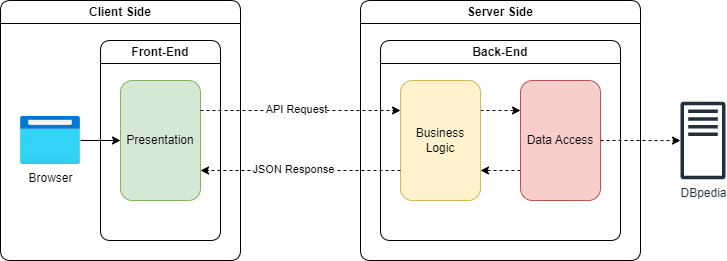
\includegraphics[height=.35\textwidth]{images/03/Architecture.drawio.png}
    \caption{Geplante Architektur des Graph Visualizers.}
    \label{fig:realization:concept:architecture}
\end{figure}

\section{Implementierung}

In diesem Kapitel wird die praktische Umsetzung des Graph Visualizer beschrieben. Aufbauend auf den in den vorherigen Kapiteln erarbeiteten Anforderungen, liegt der Schwerpunkt dieses Kapitels auf der konkreten Implementierung der Features. Das Kapitel ist nach den zentralen Funktionalitäten der Anwendung strukturiert. Innerhalb dieser Kapitel wird dann jeweils auf die Implementierung im Front- und Backend eingeganen, je nach relevanz. Ziel ist es, die Techniken und Ansätze zu erläutern, die verwendet wurden, um die Anwendung mit all ihren Anforderungen zu realisieren.

\subsection{Initialisierung der Anwendung}

Die Initialisierung der Anwendung begann mit der Einrichtung der beiden zentralen Komponenten. Der Svelte-Anwendung für das Frontend und der ASP.NET Core-Anwendung für das Backend.

Zunächst wurde die Svelte-Anwendung erstellt, die als Frontend des Graph Visualizer dient. Hierfür wurde ein neues Svelte-Projekt mit dem Svelte-CLI-Tool initialisiert. Diese Initialisierung legte die grundlegende Verzeichnisstruktur und die erforderlichen Konfigurationsdateien fest, die für die Entwicklung einer Single Page Application (SPA) notwendig sind. Im Anschluss daran wurden die benötigten Abhängigkeiten installiert. Dazu gehörten TailwindCSS für das Styling und DaisyUI als ergänzende UI-Komponentenbibliothek. Zudem wurde D3.js integriert, um die Visualisierung der Knowledge Graphen zu ermöglichen. Diese Bibliotheken wurden hinzugefügt, um die Entwicklung einer interaktiven und benutzerfreundlichen Oberfläche zu unterstützen.

Parallel dazu wurde eine ASP.NET Core-Anwendung initialisiert, die das Backend des Systems bildet. Diese Anwendung wurde mit dem .NET CLI-Tool erstellt, das eine Standard-Verzeichnisstruktur und grundlegende Konfigurationsdateien bereitstellt. Das Backend ist dafür verantwortlich, die Svelte-Anwendung auszuliefern und API-Endpunkte für die Datenverarbeitung bereitzustellen.

Um die Integration zwischen Frontend und Backend zu realisieren, wurde Vite so konfiguriert, dass es die Svelte-Anwendung kompiliert und die generierten Dateien, in das wwwroot-Verzeichnis der ASP.NET Core-Anwendung platziert. Diese Dateien werden dann von der ASP.NET Core-Anwendung als statische Dateien ausgeliefert.

Um die Auslieferung der statischen Dateien zu ermöglichen, wurden in der Startup.cs-Datei der ASP.NET Core-Anwendung die Middleware-Komponenten \textit{app.UseDefaultFiles()} und \textit{app.UseStaticFiles()} konfiguriert. Diese Middleware sorgt dafür, dass Anfragen an den Server automatisch die entsprechenden Dateien aus dem wwwroot-Verzeichnis laden und an den Client ausliefern.

Nachdem die Konfiguration abgeschlossen war, wurde die ASP.NET Core-Anwendung gestartet, um sicherzustellen, dass die Svelte-Anwendung korrekt ausgeliefert wird. Bei einem Zugriff auf den Server durch den Browser wurde die Anwendung wie erwartet geladen, was den erfolgreichen Abschluss der Initialisierung bestätigte. Diese Schritte legten die Grundlage für die weitere Implementierung der spezifischen Features des Graph Visualizer.

\subsection{Implementierung der Startseite}

Die Implementierung der Startseite des Graph Visualizer legt besonderen Wert auf eine minimalistische und benutzerfreundliche Gestaltung, um den Nutzer sofort auf den Hauptzweck der Anwendung zu fokussieren. Dies entspricht der in den nicht-funktionalen Anforderungen (\hyperref[NFR05]{NFR05}) festgelegten Priorität auf Benutzerfreundlichkeit.

Als erstes wurde das Layout der Startseite so entworfen, dass die Benutzer nur mit den notwendigsten Elementen interagieren müssen. Im Zentrum der Seite befindet sich ein auffälliges Suchfeld, das zur Eingabe von Suchbegriffen dient. Diese Reduktion auf das Wesentliche soll sicherstellen, dass die Benutzer direkt zur Hauptfunktion der Anwendung geführt werden, nämlich der Visualisierung von Knowledge Graphen. Die Startseite ist in Abbildung \ref{fig:realization:implementation:homepage} dargestellt.

\begin{figure}[h]
    \centering
    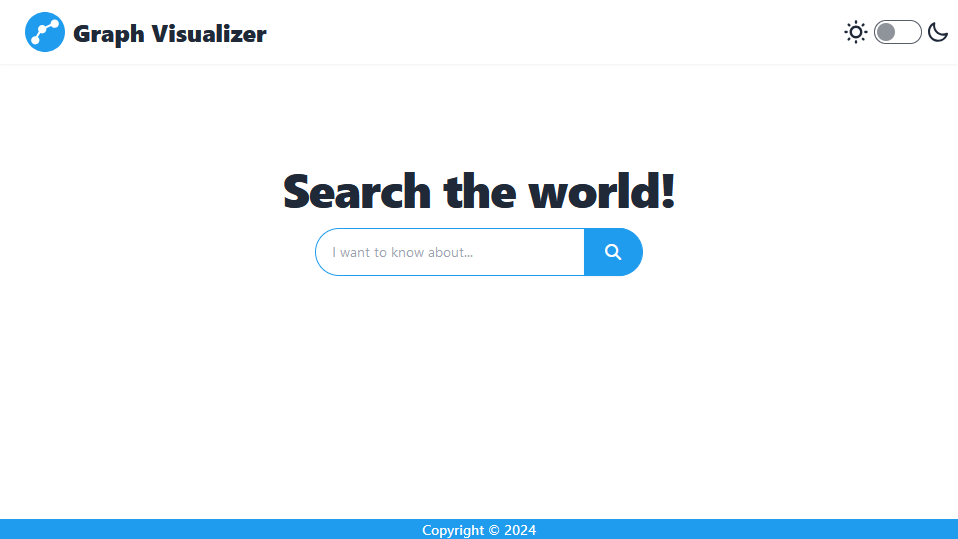
\includegraphics[height=.5\textwidth]{images/03/HomePage.png}
    \caption{Startseite des Graph Visualizers.}
    \label{fig:realization:implementation:homepage}
\end{figure}

Ein Feature der Startseite und der gesamten Anwendung ist die Unterstützung eines Dark Modes. Diese Funktion wurde implementiert, um den Komfort für die Benutzer zu erhöhen, insbesondere bei längeren Nutzungszeiten oder in Umgebungen mit schwacher Beleuchtung. Durch einen Schalter in der oberen rechten Ecke der Seite kann der Benutzer zwischen dem hellen und dunklen Modus wechseln. Dies sorgt für eine angenehmere visuelle Erfahrung und unterstützt das Ziel, einer anpassbaren und benutzerfreundlichen Oberfläche. Das Feature ist in Abbildung \ref{fig:realization:implementation:homepagedark} zu sehen.

\begin{figure}[h]
    \centering
    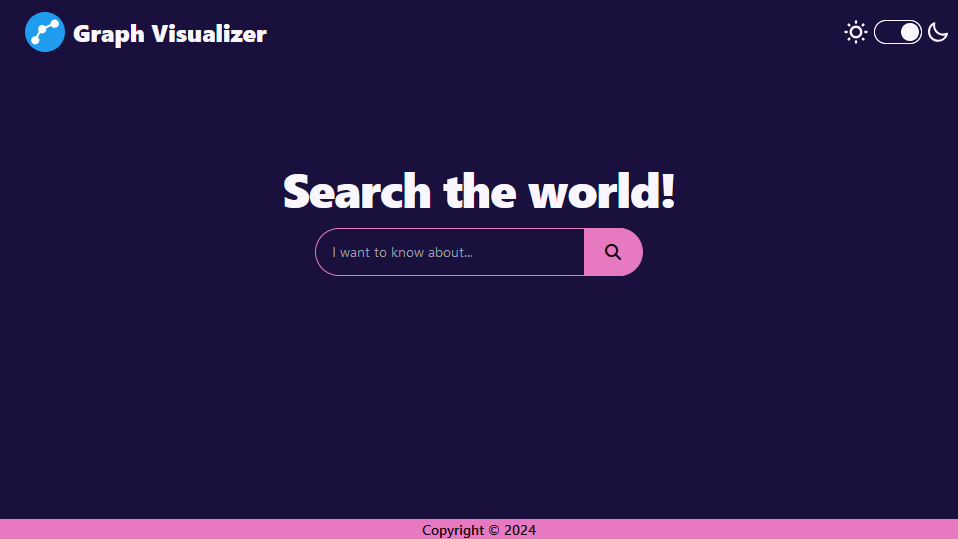
\includegraphics[height=.5\textwidth]{images/03/HomePageDark.png}
    \caption{Startseite des Graph Visualizers im Dark Mode.}
    \label{fig:realization:implementation:homepagedark}
\end{figure}

Wenn der Benutzer einen Suchbegriff in das Eingabefeld eingibt und die Suche ausführt, wird er automatisch auf die Suchseite weitergeleitet. Die URL der Suchseite enthält den Suchbegriff als Parameter (z.B. \textit{/\#/search?query=Space\%20Center}). Bereits beim Aufbau der Suchseite wird im Hintergrund eine Anfrage an den Search Endpunkt des SparqlControllers im ASP.NET Core Backend gestellt. Dieser Controller verwendet das SparqlRepository, das mithilfe des SparqlQueryClient aus der Bibliothek dotNetRdf.Core eine SPARQL-Abfrage an den DBpedia-Endpunkt sendet.

\begin{lstlisting}[caption={SPARQL-Abfrage zur Filterung von Ressourcen anhand des Labels}, label={list:realization:implementation:searchquery}]
PREFIX rdfs: <http://www.w3.org/2000/01/rdf-schema#>

SELECT DISTINCT ?resource ?label WHERE {
  ?resource rdfs:label ?label .
  FILTER(regex(?label, "{searchTerm}", "i") && langMatches(lang(?label),"EN"))
}
LIMIT 100
\end{lstlisting}

In der Abfrage aus Listing \ref{list:realization:implementation:searchquery} wird zunächst jede Ressource (\textit{?resource}) identifiziert, die ein Label (\textit{?label}) besitzt. Der FILTER-Ausdruck sorgt dafür, dass nur solche Labels berücksichtigt werden, die dem eingegebenen Suchbegriff entsprechen. Zusätzlich werden die Ergebnisse auf Labels in englischer Sprache eingeschränkt, um eine kontinuität für dieses Projekt zu erreichen. Schließlich wird die Anzahl der zurückgegebenen Ergebnisse auf 100 beschränkt, um die Performance der Abfrage zu verbessern.

Die Ergebnisse dieser Abfrage bestehen aus einer Liste von Ressourcen (URI) und ihren entsprechenden Labels, die dann in eine JSON-Struktur umgewandelt und an das Frontend übermittelt werden. Auf der Suchseite werden diese Ergebnisse als klickbare Links angezeigt, die den Benutzer weiter in die Exploration des Knowledge Graphen führen können. Diese Darstellung ist in der Abbildung \ref{fig:realization:implementation:searchpage} zu sehen.

\begin{figure}[h]
    \centering
    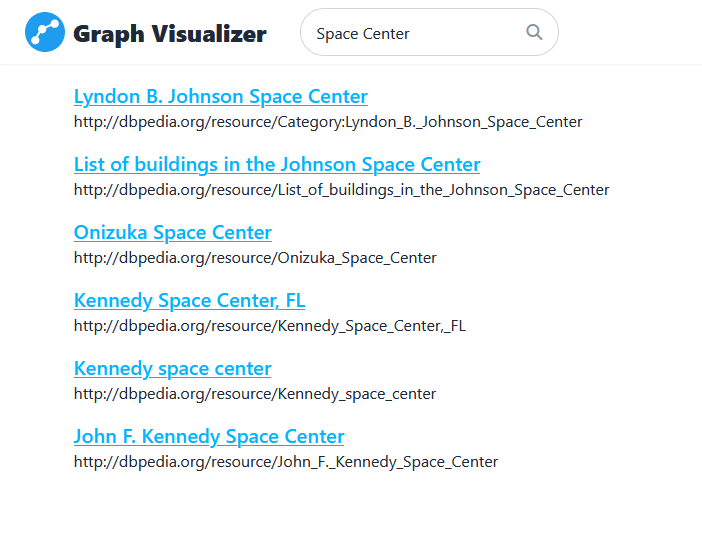
\includegraphics[height=.8\textwidth]{images/03/SearchResults.png}
    \caption{Suchseite des Graph Visualizers.}
    \label{fig:realization:implementation:searchpage}
\end{figure}

\subsection{Implementierung der Graph-View}

Die Graph-View ist das zentrale Element des Graph Visualizer und ermöglicht dem Benutzer die interaktive Erkundung von Knowledge Graphen. Die Seite bietet dem Benutzer verschiedene Optionen, um die Darstellung des Graphen anzupassen und die Daten zu filtern, um eine möglichst intuitive und effiziente Visualisierung zu gewährleisten.

\subsubsection{Aufbau der Graph-View}

Die Graph-View stellt den zentralen Bereich der Anwendung dar, in dem die Visualisierung des Knowledge Graphen erfolgt. Diese Ansicht ermöglicht es dem Benutzer, den Graphen interaktiv zu erkunden und anzupassen. Auf der linken Seite befindet sich ein Bedienfeld, das verschiedene Einstellungsmöglichkeiten bietet, um die Darstellung und das Verhalten des Graphen zu beeinflussen. Die Graph-View ist in Abbildung \ref{fig:realization:implementation:graphview} dargestellt.

\begin{figure}[h]
    \centering
    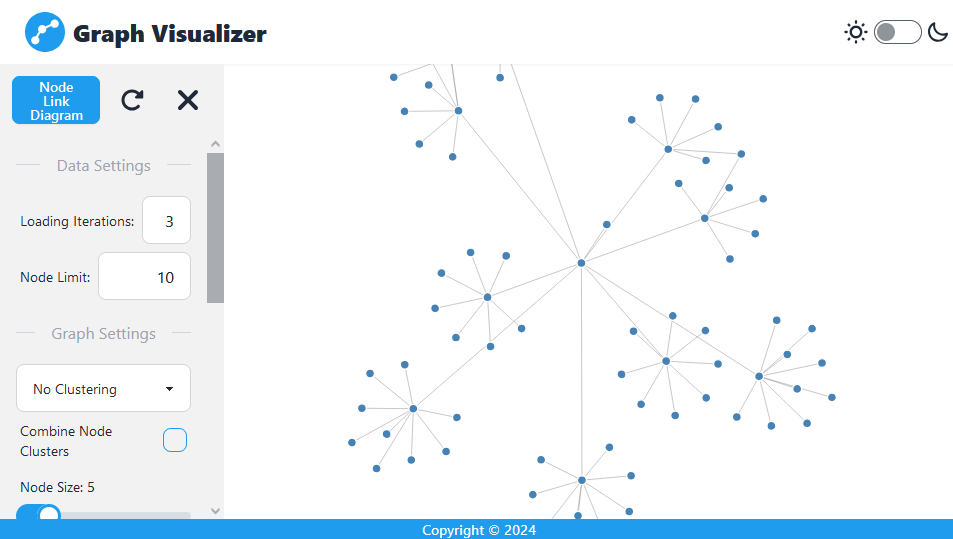
\includegraphics[height=.5\textwidth]{images/03/GraphView.png}
    \caption{Graph-View des Graph Visualizers.}
    \label{fig:realization:implementation:graphview}
\end{figure}

In dem Menu auf der linken Seite gibt es mehrere Panels mit unterschiedlichen Einstellungen. Zu den Data Settings gehört die Möglichkeit, die Anzahl der Ladeiterationen sowie das Knotenlimit festzulegen. Diese Einstellungen bestimmen, wie tief der Graph geladen wird und wie viele Knoten gleichzeitig dargestellt werden. Diese Parameter erlauben es die Performance der Anwendung zu kontrollieren und zu testen, welche Techniken zu einer Leistungssteigerung der Anwendung führen.

Der Graph selbst wird standardmäßig als Node-Link Diagramm dargestellt, da es eine intuitive Visualierung der Beziehungen und der Knoten bietet. Auf die Erstellung des Graphen wird in Kapitel \ref{realization:implementation:graphDrawing} noch genauer eingeganen.

\subsubsection{Laden des Graphen}

Beim Laden der Graph-View wird die URI der Ressource aus der URL extrahiert (z.B. \textit{/\#/graph/?uri=http://dbpedia.org/resource/Kennedy\_Space\_Center,\_FL}). Diese URI wird an das Backend übermittelt, das den entsprechenden Graphen von DBpedia abruft und als JSON an das Frontend zurückgibt. Das Abrufen des Graphen geschieht im Backend, da es eine bessere Performance bietet. Das parallele Abrufen von Ressourcen beschleunigt das Laden großer Graphen deutlich. Ein zentraler Bestandteil dieses Prozesses ist die Get-Methode des SparqlRepository. Diese Methode übernimmt die Aufgabe, den Graphen zu laden und ihn für die Anzeige vorzubereiten.

Ein wichtiger Bestandteil der Implementierung ist der Cache, der zur Verbesserung der Performance dient. Der Cache speichert zuvor geladene Graphen, um unnötige Anfragen an die externe Datenquelle zu vermeiden. Wenn eine Anfrage an das Backend gestellt wird, prüft die Get-Methode zunächst, ob der angeforderte Graph bereits im Cache vorhanden ist. Falls der Graph im Cache vorhanden ist, wird er direkt aus dem Cache zurückgegeben, was die Ladezeit erheblich verkürzt. Ist der Graph jedoch nicht im Cache vorhanden, wird er mittels der \textit{LoadGraphAsync} Methode von DBpedia abgerufen und anschließend in den Cache aufgenommen.

Der Einsatz eines Caches kann die Performance der Anwendung signifikant verbessern, insbesondere wenn häufig auf dieselben Graphen zugegriffen wird. Allerdings ist der Speicherplatz des Caches begrenzt, und bei sehr großen Datenmengen könnte der Cache an seine Grenzen stoßen. In einer produktiven Umgebung könnte es daher sinnvoll sein, eine dedizierte Datenbank zur Zwischenspeicherung der Graphen zu verwenden, um eine noch robustere Lösung zu bieten.

code einfügen

\subsubsection{Erweiterung des Graphen}

Zusätzlich zum primären Graphen kann die Anwendung auch Subgraphen laden. Dies ist sogar notwendig, um einen \enquote{echten} Knowledge Graphen zu erhalten. Wenn ein Graph aus der DBpedia-Datenbank geladen wird, wird die angeforderte Ressource inklusive all ihrer direkten Links und Informationen abgerufen. Das entspricht einem zentralen Knoten und seinen Verbindungen zu anderen Ressourcen. Ein solcher Graph ist in Abbildung \ref{fig:realization:implementation:simpleGraph} dargestellt.

\begin{figure}[h]
    \centering
    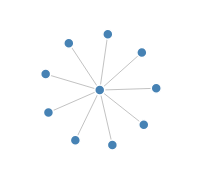
\includegraphics[height=.3\textwidth]{images/03/SimpleGraph.png}
    \caption{Visualierung einer Ressource von DBpedia.}
    \label{fig:realization:implementation:simpleGraph}
\end{figure}

Diese Darstellung ist sicherlich nicht, das was man sich unter einem großen Knowledge Graphen vorgestellt. Um diesen zu erhalten, muss man die Ressourcen, mit welchen der Graph verbunden ist abgerufen und den originalen Graphen um diese Informationen erweitern.

Die Methode LoadSubGraphsAsync wird verwendet, um diese weiterführenden Ressourcen zu laden und in den bestehenden Graphen zu integrieren. Diese Methode lädt die verknüpften Ressourcen, indem sie für jede verlinkte Ressource erneut die Get-Methode aufruft. Die geladenen Subgraphen werden dann in den ursprünglichen Graphen integriert. Dieser rekursive Prozess ermöglicht es dem Benutzer, die Exploration des Knowledge Graphen zu vertiefen und weitere Verbindungen und Zusammenhänge zu entdecken, ohne dabei die Übersichtlichkeit zu verlieren.

code einfügen

Durch diese Herangehensweise beim Abrufen des Graphen stellt die Implementierung sicher, dass komplexe Netzwerke effizient geladen werden können.

\subsection{Implementierung der Graph-Visualisierungen}
\label{realization:implementation:graphDrawing}

Die Implementierung der Graph-Visualisierungen im Graph Visualizer umfasst zwei wesentliche Diagrammarten. Das Node-Link Diagramm und die Adjazenzmatrix. Diese beiden Visualisierungstechniken bieten unterschiedliche Perspektiven auf die zugrunde liegenden Daten und ermöglichen eine flexible Analyse von Knowledge Graphen. Bevor jedoch die Implementierung dieser Diagramme beschrieben wird, ist es wichtig, die Struktur der vom Backend gelieferten Daten zu verstehen und wie diese Daten für die Visualisierung aufbereitet werden müssen.

\subsubsection{Datenstruktur und Aufbereitung}

Die Daten, die vom Backend an das Frontend übermittelt werden, bestehen aus einer Liste von Knoten, die als JSON formatiert sind. Jeder Knoten enthält die folgenden Attribute:

\begin{itemize}
    \item Uri: Die eindeutige Ressource-Identifier-URI des Knotens.
    \item Label: Ein menschenlesbarer Name oder Titel, der den Knoten beschreibt.
    \item Properties: Ein Dictionary von Eigenschaften, das zusätzliche Informationen über den Knoten enthält. Die Schlüssel im Wörterbuch sind die Namen der Eigenschaften, und die Werte sind die entsprechenden Inhalte.
    \item Links: Ein Dictionary, das Verbindungen zu anderen Knoten beschreibt. Die Schlüssel sind die Typen der Verbindungen, und die Werte sind Listen von URIs, die auf die verlinkten Knoten verweisen.
\end{itemize}

Ein solcher Knoten im JSON Format ist in Listing \ref{list:realization:implementation:nodejson} dargestellt.

\begin{lstlisting}[caption={Informationen einer Node im JSON Format.}, label={list:realization:implementation:nodejson}]
{
    "Uri": "http://dbpedia.org/resource/Kennedy_Space_Center,_FL",
    "Label": "Kennedy Space Center",
    "Properties": {
        "Location": "Florida",
        "Operator": "NASA"
    },
    "Links": {
        "located_in": ["http://dbpedia.org/resource/Florida"],
        "operated_by": ["http://dbpedia.org/resource/NASA"]
    }
}
\end{lstlisting}

Damit diese Daten von D3.js für die Visualisierung genutzt werden können, müssen sie zunächst in ein Format umgewandelt werden, das die Bibliothek versteht. Für das Node-Link Diagramm bedeutet dies, dass die Knoten und die Kanten extrahiert und entsprechend strukturiert werden müssen. Ein Beispiel für die Transformierten Daten ist in Listing \ref{list:realization:implementation:nodesAndLinksJson} dargestellt.

\begin{lstlisting}[caption={Informationen einer Node im JSON Format.}, label={list:realization:implementation:nodesAndLinksJson}]
    const nodes = [
        { id: "http://dbpedia.org/resource/Kennedy_Space_Center,_FL", label: "Kennedy Space Center" },
        { id: "http://dbpedia.org/resource/Florida", label: "Florida" },
        { id: "http://dbpedia.org/resource/NASA", label: "NASA" }
    ];
    
    const links = [
        { source: "http://dbpedia.org/resource/Kennedy_Space_Center,_FL", target: "http://dbpedia.org/resource/Florida", type: "located_in" },
        { source: "http://dbpedia.org/resource/Kennedy_Space_Center,_FL", target: "http://dbpedia.org/resource/NASA", type: "operated_by" }
    ];
\end{lstlisting}

Diese Datenstruktur ermöglicht es D3.js, Knoten und Verbindungen darzustellen, wobei jeder Knoten durch eine eindeutige id identifiziert wird und die Kanten durch Quell- und Ziel-Eigenschaften spezifiziert sind.

\subsubsection{Node-Link Diagramm}

Das Node-Link Diagramm ist eine der zentralen Visualisierungsformen des Graph Visualizer und stellt die Beziehungen zwischen den Entitäten eines Knowledge Graphen intuitiv und visuell ansprechend dar. Die Implementierung des Node-Link Diagramms erfolgt mittels D3.js. Die Knoten werden als Kreise dargestellt, deren Positionen durch ein Force-Directed Layout bestimmt werden. Dieses Layout modelliert die Knoten als physikalische Objekte, die durch Kräfte zueinander in Beziehung stehen, ähnlich wie Federn und Ladungen in einem physikalischen Modell. Knoten, die durch Kanten verbunden sind, werden durch diese Kräfte näher zusammengeführt, während unverbundene Knoten weiter auseinanderliegen. Die Oberfläche ist in Abbildung \ref{fig:realization:implementation:GraphViewWithSettings} dargestellt.

\begin{figure}[h]
    \centering
    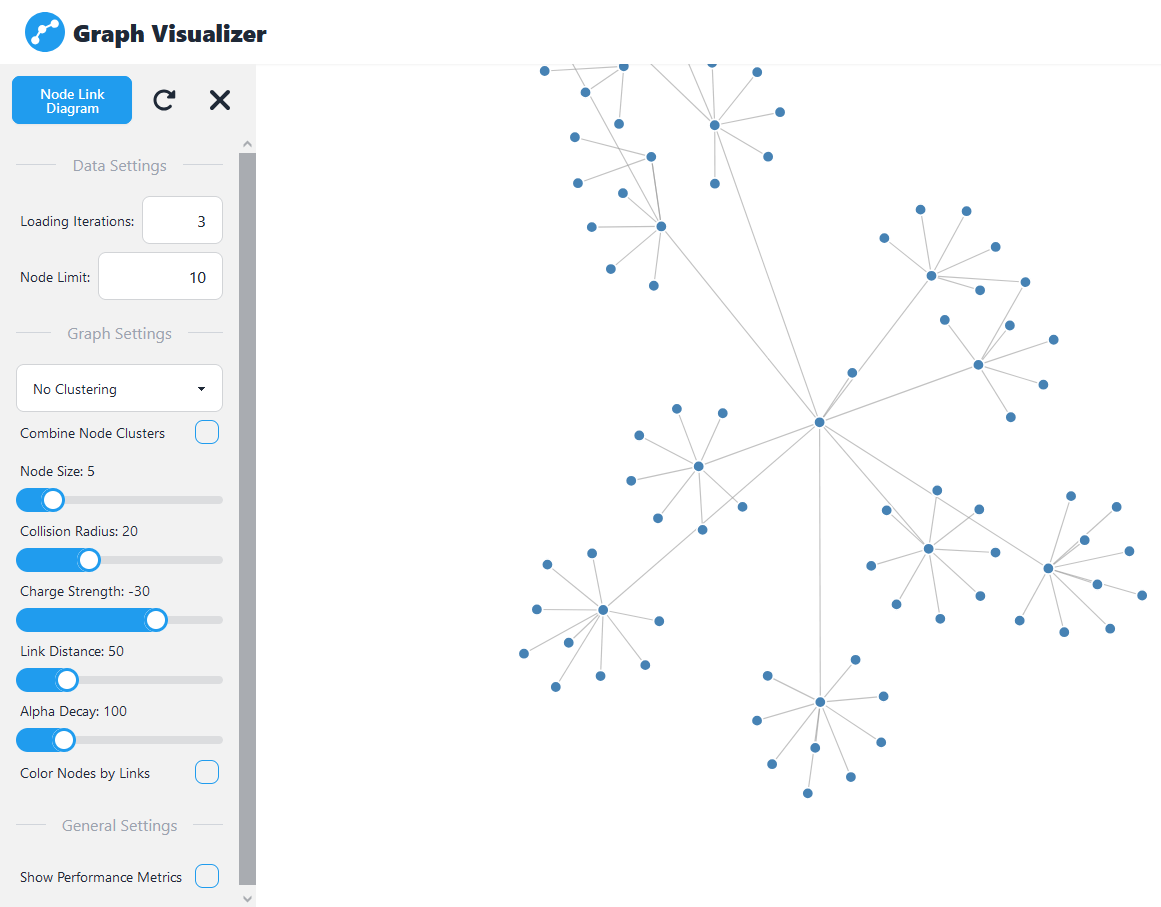
\includegraphics[height=.5\textwidth]{images/03/GraphViewWithSettings.png}
    \caption{Oberfläche des Graph Visualizers mit Node-Link Diagramm.}
    \label{fig:realization:implementation:GraphViewWithSettings}
\end{figure}

Die Darstellung der Knoten und Kanten im Node-Link Diagramm kann durch verschiedene Einstellungen im \enquote{Graph Settings}-Panel angepasst werden. Hier können die Benutzer die Größe der Knoten, den Kollisionsradius, die Ladungsstärke und die Link-Distanz konfigurieren. Die Größe der Knoten bestimmt, wie prominent die einzelnen Entitäten im Diagramm erscheinen, während der Kollisionsradius beeinflusst, wie nah die Knoten zueinander liegen dürfen, bevor sie sich abstoßen. Die Ladungsstärke reguliert die Abstoßungskraft zwischen den Knoten, was bei der Entzerrung dicht verbundener Bereiche des Graphen hilfreich ist. Die Link-Distanz steuert die Länge der Verbindungen zwischen den Knoten, was die Gesamtstruktur des Graphen entweder dichter oder weiter gefasst erscheinen lässt. Das Ergebnis einer Änderung der Einstellungen ist in Abbildung \ref{fig:realization:implementation:NodeLinkWithChangedSettings} zu sehen.

\begin{figure}[h]
    \centering
    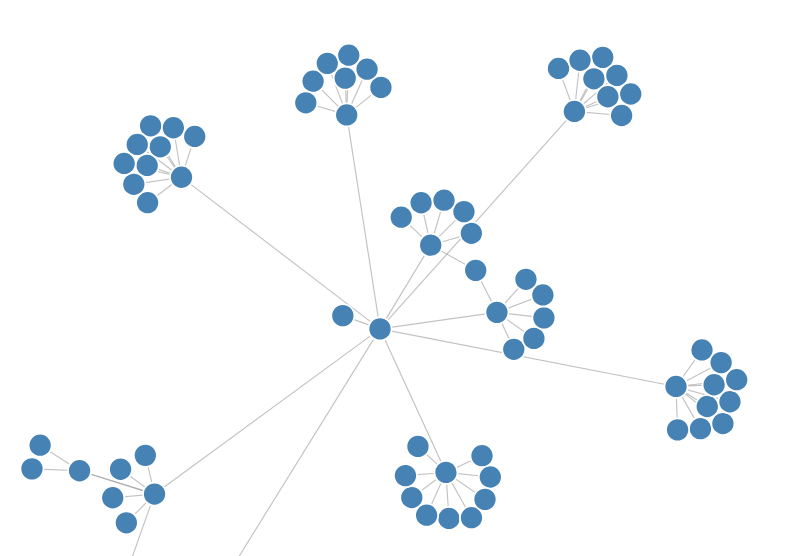
\includegraphics[height=.5\textwidth]{images/03/NodeLinkChangedSettings.png}
    \caption{Node Link Diagramm mit veänderten Einstellungen.}
    \label{fig:realization:implementation:NodeLinkWithChangedSettings}
\end{figure}

Eine weitere Einstellung ist die Farbgebung der Knoten. Um die Visualisierung zugänglicher zu machen, wurde eine Option eingebaut, die es ermöglicht die Farbe der Knoten basierend auf der Anzahl Verbindungen berechnen zu lassen. Durch die Farbgebung können Benutzer auf einen Blick erkennen, welche Knoten besonders stark vernetzt sind oder spezifische Verbindungen aufweisen. Ein Beispiel hierfür ist in Abbildung \ref{fig:realization:implementation:ColorNodesByLinks} dargestellt.

\begin{figure}[h]
    \centering
    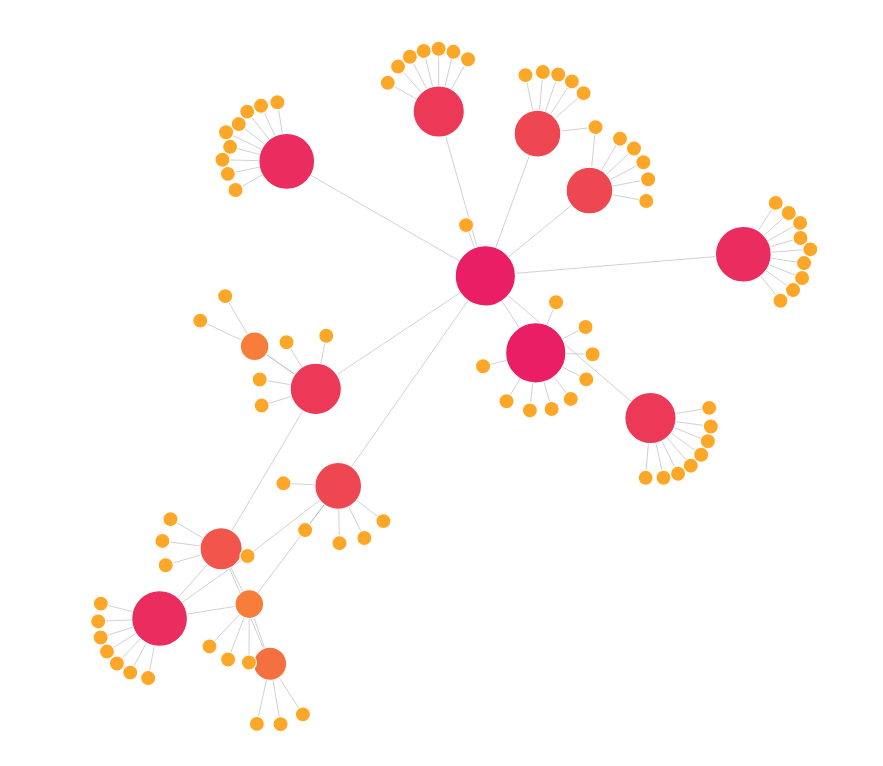
\includegraphics[height=.5\textwidth]{images/03/ColorNodesByLinks.png}
    \caption{Node Link Diagramm mit der Einstellung \enquote{Color Nodes by Links}.}
    \label{fig:realization:implementation:ColorNodesByLinks}
\end{figure}

Zusätzlich ist die Einstellung Alpha Decay ein wesentlicher Parameter, der die Stabilisierung des Force-Directed Layouts beeinflusst. Dieser Wert bestimmt, wie schnell das Layout konvergiert und zur Ruhe kommt. Ein hoher Alpha Decay-Wert sorgt dafür, dass sich das Layout schneller stabilisiert, was bei der Visualisierung großer Graphen von Vorteil sein kann, da die Knotenpositionen rascher endgültig festgelegt werden. Andererseits, kann die Darstellung dann unübersichtlicher sein, als bei einer Simulation die länger läuft. Diese Diskrepanz ist in den Abbildungen \ref{fig:realization:implementation:NodeLinkLowAlpha} und \ref{fig:realization:implementation:NodeLinkHighAlpha} dargestellt. In der linken Abbildung wurde der Simulation viel Zeit gegeben, während die rechte Darstellung einen hohen Alpha Decay hatte. Hier Zeigt sich deutlich, dass das Zentrum der rechten Darstellung deutlich unübersichtlicher ist.

\begin{figure}
    \centering
    \begin{minipage}{.5\textwidth}
        \centering
        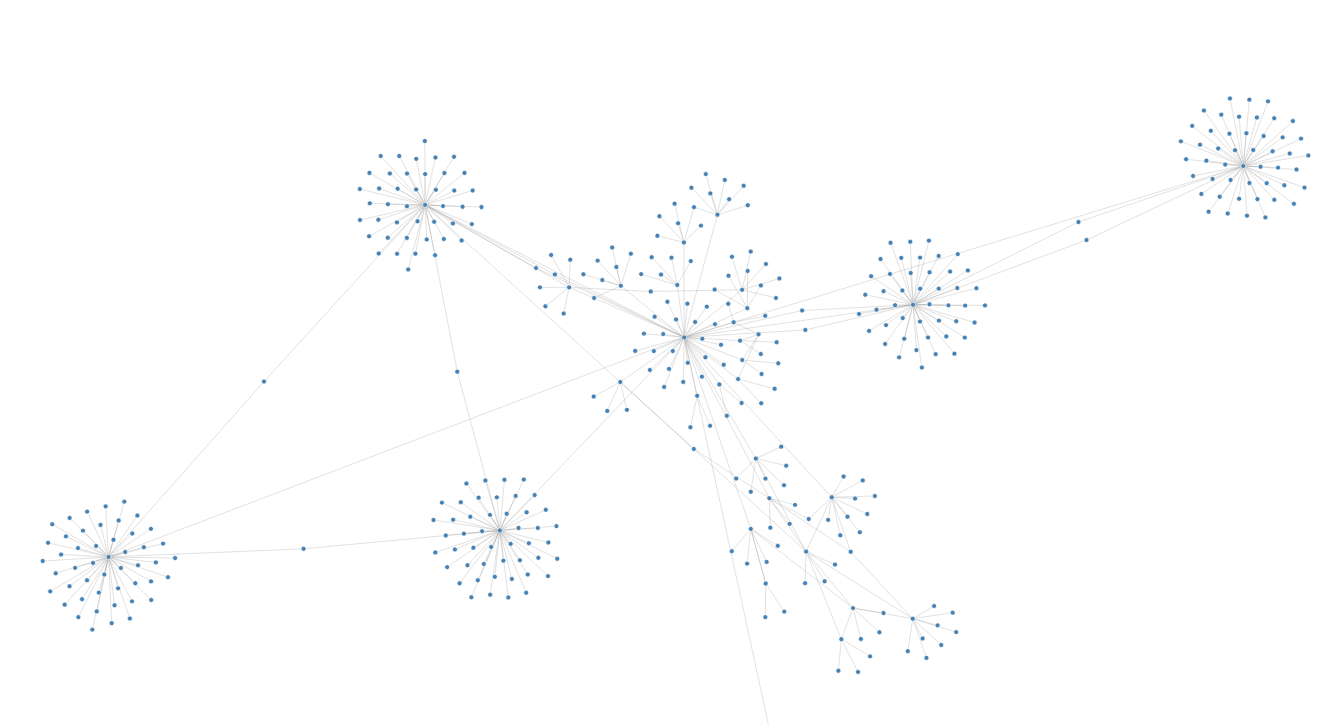
\includegraphics[width=1\linewidth]{images/03/NodeLinkLowAlpha.png}
        \caption{Node Link Diagramm niedrigem Aplha Decay.}
        \label{fig:realization:implementation:NodeLinkLowAlpha}
    \end{minipage}%
    \begin{minipage}{.5\textwidth}
        \centering
        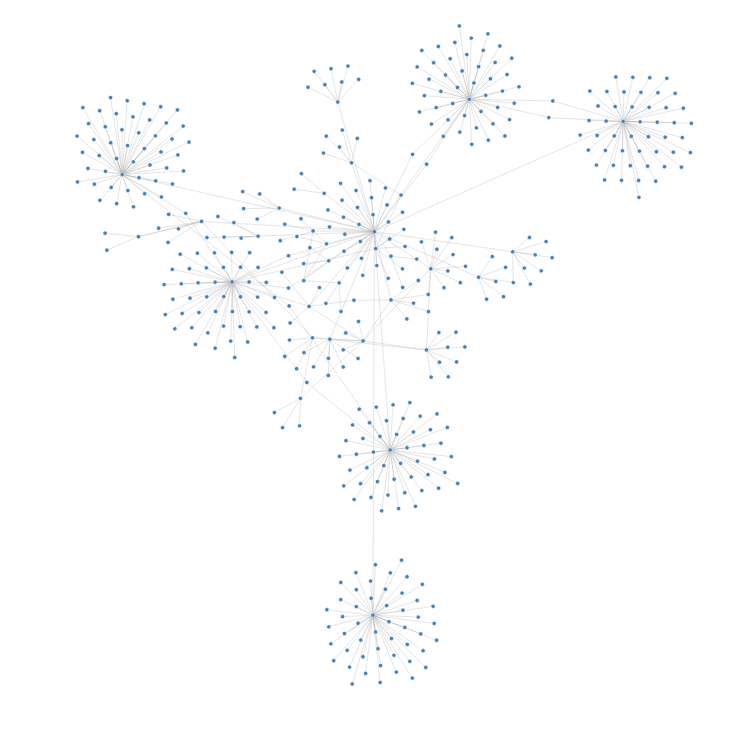
\includegraphics[width=1\linewidth]{images/03/NodeLinkHighAlpha.png}
        \caption{Node Link Diagramm hohem Aplha Decay.}
        \label{fig:realization:implementation:NodeLinkHighAlpha}
    \end{minipage}
\end{figure}

Die umfangreichen Anpassungsmöglichkeiten des Node-Link Diagramms sind darauf ausgelegt, die in den nicht-funktionalen Anforderungen definierten Ziele zu erreichen. Dazu gehört unter anderem die Forderung nach einer hohen Benutzerfreundlichkeit und Flexibilität bei der Darstellung von komplexen Knowledge Graphen. Die interaktiven Anpassungsoptionen ermöglichen es den Benutzern, das Diagramm an ihre spezifischen Bedürfnisse anzupassen, was insbesondere bei der Analyse großer und komplexer Graphen von entscheidender Bedeutung ist.

\subsubsection{Adjazenzmatrix}

Die Adjazenzmatrix ist eine alternative Visualisierungsmethode, die sich besonders für die Analyse von großen und komplexen Graphen eignet, bei denen die Verbindungen zwischen den Knoten im Vordergrund stehen. In einer Adjazenzmatrix werden die Knoten sowohl in den Zeilen als auch in den Spalten einer Matrix angeordnet. Jede Zelle der Matrix repräsentiert eine mögliche Verbindung zwischen den Knoten, die durch die entsprechende Zeile und Spalte definiert sind. Ist eine Verbindung vorhanden, wird die Zelle entsprechend markiert. Diese Visualisierungsmethode eignet sich besonders gut, um Cluster und dichte Netzwerke innerhalb des Graphen schnell zu identifizieren. Durch die Anordnung der Knoten in einer Matrix können Verbindungen direkt und ohne Überlappungen dargestellt werden, was bei komplexen Graphen mit vielen Knoten und Kanten eine deutlich verbesserte Lesbarkeit ermöglicht. Der Nutzer kann im Graph Visualizer über das Settings-Panel auf die Adjazenzmatrixdarstellung umschalten. Diese Darstellung ist in Abbildung \ref{fig:realization:implementation:AdjacencyMatrixView} zu sehen.

\begin{figure}[h]
    \centering
    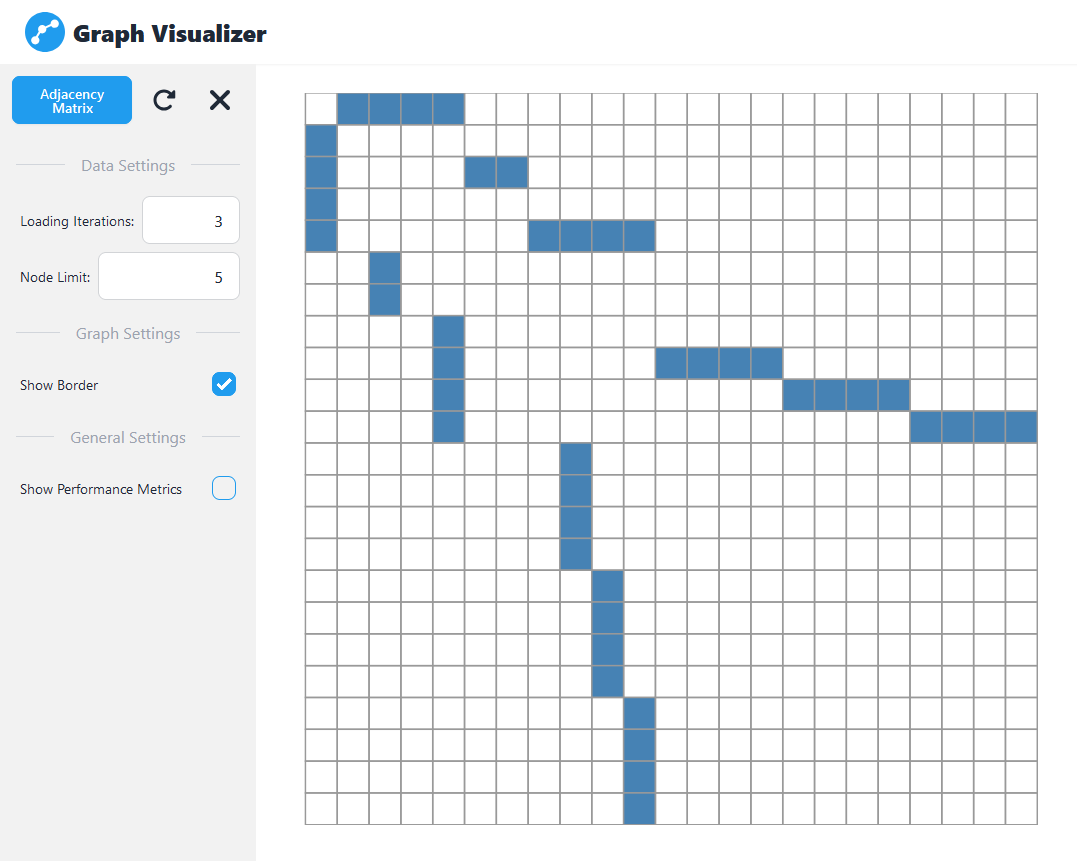
\includegraphics[height=.5\textwidth]{images/03/AdjacencyViewWithSettings.png}
    \caption{Adjazenzmatrixdarstellung im Graph Visualizer.}
    \label{fig:realization:implementation:AdjacencyMatrixView}
\end{figure}

Die Adjazenzmatrix im Graph Visualizer bietet nur eine Anpassungsmöglichkeit. Sie ermöglicht es die Umrandung der Zellen ein- oder auszuschalten. Die Anzeige der Umrandung hilft dabei, die einzelnen Zellen klar voneinander zu trennen, was besonders bei dichten Graphen nützlich ist. Die Darstellung der Trennlinien kostet aber auch Performance, weshalb dem Nutzer die Möglichkeit gegeben wird diese auszuschalten.

Die Adjazenzmatrix erfüllt mehrere der im Projekt definierten Anforderungen, insbesondere in Bezug auf die Darstellung komplexer Netzwerkstrukturen und die Benutzerfreundlichkeit. Durch die klare und strukturierte Darstellung von Verbindungen ermöglicht die Adjazenzmatrix eine einfache Identifikation von Clustern und Mustern im Graphen, was die Analyse und das Verständnis der zugrunde liegenden Daten erheblich erleichtert.

\section{Vergleich}
\label{realization:comparison}

\chapter{Zusammenfassung und Ausblick}